\newpage
\section{Intégration continue}
L'intégration continue (CI) est une pratique de développement logiciel visant à automatiser et à faciliter le processus de construction et de tests d'une application.

Diagfit est construit et testé sur la plate-forme de gestion de développement GitLab à l'aide d'une série de tâches automatisées, appelées "jobs", qui sont exécutées séquentiellement en réponse aux changements du code source.

\todo{intro qui dit integration continue et mon role dedans}
\todo{remonter la mission confiée avec les pb avant et nouveau}

\subsection{Technologies utilisées}
\subsubsection{Docker}
Docker est une plate-forme de "conteneurisation" légère qui permet de créer, gérer et exécuter des applications dans des conteneurs.
Les conteneurs Docker encapsulent le code, les bibliothèques et les dépendances d'une application, garantissent une exécution cohérente et prévisible quel que soit l'environnement.
Contrairement aux machines virtuelles traditionnelles, les conteneurs partagent le noyau du système hôte, ce qui les rend plus efficaces en termes de ressources.

L'un des avantages clés de Docker est sa portabilité.
Un fichier descriptif unique, appelé "dockerfile", est responsable de la création de l'image, il est ensuite possible de créer un processus basé sur les fichiers, executables et sur l'environnement définis dans cette image.
Ce processus est appelé container.
Grâce à Docker, on peut empaqueter votre application ainsi que ses dépendances dans un conteneur unique, puis le déplacer sans effort entre différents environnements tels qu'un ordinateur portable de développement, un serveur de production ou un cloud public.

Docker utilise des images pour définir le contenu et la configuration d'un conteneur.
Les images Docker sont des modèles immuables qui contiennent tout ce dont un conteneur a besoin pour s'exécuter.
Lorsqu'un fichier décrivant une image est modifié, seule la partie modifiée et ce qui suit est reconstruit, en réutilisant ce qui avait été précédemment construit.

\subsubsection{Docker Compose}
Docker Compose est un outil simplifiant la gestion d'applications composées de plusieurs conteneurs.
Plutôt que de nécessiter une gestion manuelle de chaque conteneur et de ses paramètres respectifs, Docker Compose offre la possibilité de définir l'ensemble de la configuration d'une application dans un fichier "docker-compose.yml".

Dans ce fichier, les services sont spécifiés, lesquels constituent les divers composants de l'application, incluant leurs images Docker, les ports exposés, les variables d'environnement et d'autres options de configuration.
En utilisant la commande docker-compose up, il est possible de créer et lancer simultanément tous les conteneurs, instaurant un environnement cohérent pour l'application.

De plus, Docker Compose simplifie la communication entre les conteneurs d'une application en mettant en place un réseau virtuel par défaut.
Ceci permet aux services de se faire référence mutuellement par leur nom de service.

\subsection{Environnement de développement}
\subsubsection{Architecture globale de Diagfit}
Les développeurs travaillent sur la dernière version en production : Diagfit 2.5.

\begin{figure}[ht!]
    \centering
    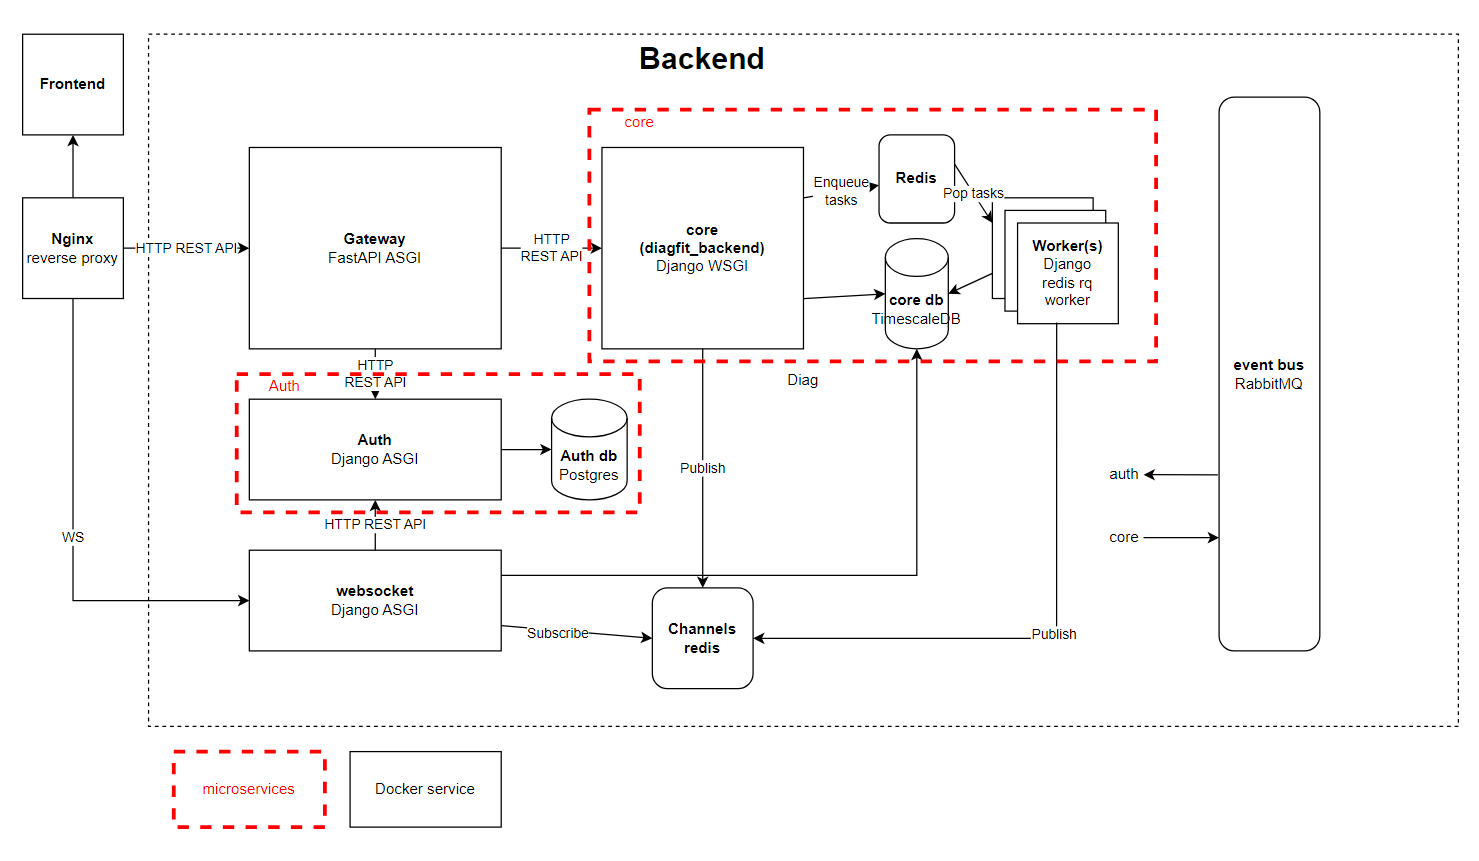
\includegraphics[width=0.9\textwidth]{paper/figures/archi2-5.png}
    \caption{Architecture globale de Diagfit 2.5}
    \label{fig:archi2-5}
\end{figure}

Ci-dessus, l'architecture globale de l'application Diagfit avec tous leurs services.
Suite à une refactorisation de l'application, le système s'est grandement simplifié.

\begin{figure}[ht!]
    \centering
    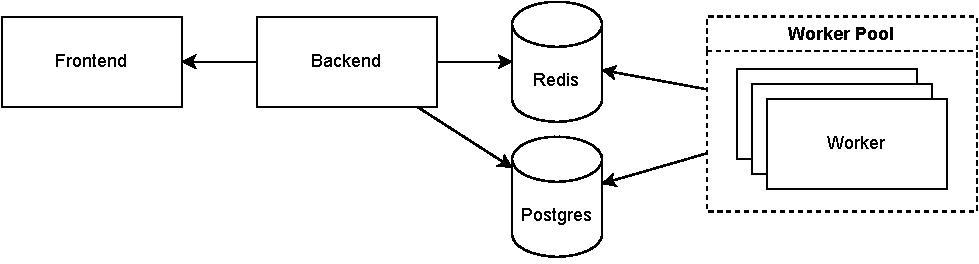
\includegraphics[width=0.66\textwidth]{paper/figures/archi2-6.pdf}
    \caption{Architecture globale du nouveau Diagfit 2.6}
    \label{fig:archi2-6}
\end{figure}

La réduction des services a permis aux développeurs de travailler avec une couche de complexité en moins tout en conservant les mêmes fonctionnalités.

D'un point de vue de l'automatisation des processus, la réduction des services est synonyme avec une réduction du temps de création des environnements.

\subsubsection{Utilisation de Docker et Docker compose}
L'image Docker utilisée pour Diagfit lors de la CI présentait une complexité considérable dans la définition de l'environnement de l'application.
Cependant, cette approche se révélait fastidieuse et entraînait des incohérences notables entre l'environnement de test local et celui généré durant la CI via GitLab.

\subsubsection{Mission confiée}
La mission qui m'a été confiée fut d'optimiser le dockerfile et le fichier Docker Compose utilisés pour le logiciel Diagfit.

J'ai aussi eu l'occasion de créer une image Docker et un fichier Docker Compose pour créer un environnement contrôlé utilisable pour la création du logiciel et également pour les tests des développeurs.

\subsection{Missions effectuées et problèmes rencontrés}
\subsubsection{Optimisation du dockerfile ci et docker compose}
L'assemblage d'une image Docker à partir d'un dockerfile se déroule en plusieurs étapes, ligne par ligne.
Lors de la reconstruction de l'image, Docker est en mesure de reprendre le processus depuis la première modification dans le fichier.

Lors de cette mission, nous avons reconnu l'importance d'une initialisation efficace de l'environnement de l'image Docker.
En effet, étant donné que le téléchargement des packages utilisés pour le logiciel était une étape longue et peu sujette au changement, il était judicieux de l'exécuter avant la récupération du code en développement.

De plus, en réduisant le nombre de services utilisés, nous avons pu éliminer certains éléments du fichier docker-compose, contribuant ainsi à accélérer le temps de lancement de l'application.

\subsubsection{Création de multiples Dockerfiles}
Dans le cadre cette mission, l'une des priorités était d'assurer une homogénéité entre l'environnement de développement sur l'ordinateur des développeurs backend et celui utilisé sur la plateforme CI de GitLab.
Pour répondre à ce besoin crucial, j'ai entrepris la création de plusieurs Dockerfiles distincts, chacun adapté à un aspect spécifique du processus de développement.

L'un des résultats significatifs de cette initiative a été la mise en place de deux images Docker distinctes : l'une conçue spécifiquement pour le rendu de l'application, et l'autre optimisée pour les phases de développement et de tests unitaires.

L'intégration de Docker dans notre flux de travail au sein de GitLab a apporté des améliorations significatives, mais elle a également nécessité des ajustements dans l'environnement de travail de la plateforme.
Lors de la transition vers une approche basée sur Docker, nous avons rencontré un défi majeur : comment gérer le processus de construction d'images de manière automatisée tout en assurant la flexibilité nécessaire pour le développement et les tests ?

Pour résoudre ce défi, nous avons mis en place un mécanisme ingénieux : nous avons introduit une image Docker générique, spécialement conçue pour la construction d'images.
Cette approche nous a permis d'automatiser la génération des images et de maintenir un niveau élevé de cohérence entre les différentes étapes du processus.

Cependant, tout ne s'est pas déroulé sans accrocs.
Lors de l'implémentation de cette nouvelle approche au sein de la CI GitLab, nous avons constaté que certaines variables définies dans le dockerfile ne s'appliquaient pas correctement aux jobs en cours d'exécution.
Après une analyse minutieuse, nous avons identifié que certaines variables étaient déjà définies au niveau de l'environnement GitLab en tant que variables globales, ce qui entraînait des conflits.
Nous avons rapidement résolu ce problème en utilisant des variables personnalisées spécifiques au programme, ce qui a permis de garantir la cohérence des configurations et d'éviter les problèmes de sécurité : la variable fixée globalement était une donnée sensible.

\subsubsection{Impacts bénéfiques}
Les changements apportés à l'environnement de développement ont eu des répercussions positives, notamment :
\begin{itemize}
    \item \textbf{Amélioration de la cohérence et de la robustesse de l'infrastructure :} L'utilisation de Docker et la restructuration de la GitLab CI ont renforcé la cohérence et la robustesse de notre infrastructure de développement.
    La séparation des images et des environnements spécifiques a considérablement réduit les risques d'incohérence entre les différentes étapes du processus.
    \item \textbf{Gains de temps pour les développeurs :} En éliminant la nécessité de recréer continuellement l'environnement de test, les développeurs ont pu économiser un temps précieux.
    Cela leur a permis de se concentrer davantage sur le développement et les tests de l'application, au lieu de perdre du temps à configurer manuellement les environnements.
    \item \textbf{Réduction du temps d'exécution des tests :} Le temps d'exécution du job de test a été réduit de 12 minutes 30 secondes à seulement 11 minutes 15 secondes.
\end{itemize}